\section*{From concert to recording}
\label{sec:concert-recording}

\input{include/ethersound-cd-url.tex}
\emph{etherSound} was commissioned in 2002 by curator Miya Yoshida for
her project \emph{The Invisible Landscapes} and was realized for the
first time in August 2003 at \emph{Malm\"{o} Art Museum} in Malm\"{o},
Sweden. Since then it has been performed on several occasions in
Sweden, Denmark, UK and the USA. The principal idea behind
\emph{etherSound} is to create a vehicle for audience collaboration in
the shape of an `instrument' that is playable by anybody who can send
SMS (Short Messages Service) messages. It is an effort to move the
initiative of making and distributing sounds from the
composer/musician to the listener. It can take on different shapes (a
performance environment, sound installation, composition tool, etc.)
but its representation on this record is perhaps the hitherto most
detached and abstract of all versions produced, in that it introduces
a distance between the performers, the listener, and the
collaborators.

As an interactive system \emph{etherSound} takes input in the form of
SMS messages from which it creates `message-scores', then transformed
to short \useGlosentry{glos:electro-mus}{electro-acoustic} `message-compositions'. Each message
received by the system gives rise to a sound event, a
`message-composition', that lasts for 15 seconds up to 2 minutes. The
length of the event depends on the relative length and complexity of
the message text. Hence a short message will be more likely to
generate a shorter message-composition than a long message, but a
short message with a couple of words with inter-punctuation may render
a longer message-composition than a long message containing only
gibberish. But also the message-composition's inherent sonic
complexity may be increased by a more complex message. The electronic
part on this recording is the result of a large number of SMS messages
contributed by collaborators during a concert performance of
\emph{etherSound} on May 8, 2004 at \emph{Jeriko} in Malm\"{o},
Sweden. In the concert, apart from myself and Peter Nilsson, Andreas
Andersson played saxophones, Anders Nilsson played guitar and David
Carlsson played the bass. Prior to our appearance, a performance of
\emph{Flight}, an electro-acoustic piece for speakers by Swedish
composer Anders Blomqvist, was scheduled. But for the audience to get
acquainted with the interface of \emph{etherSound}, the system was
responding to messages also \emph{before} Blomqvist's
\emph{Flight}. In total over one hundred messages were received in
the period from the beginning of the concert (including the
pre-concert time) until the end of our performance; a time span of
about one hour.

\begin{wrapfigure}{r}{0.4\linewidth}
  \centering
  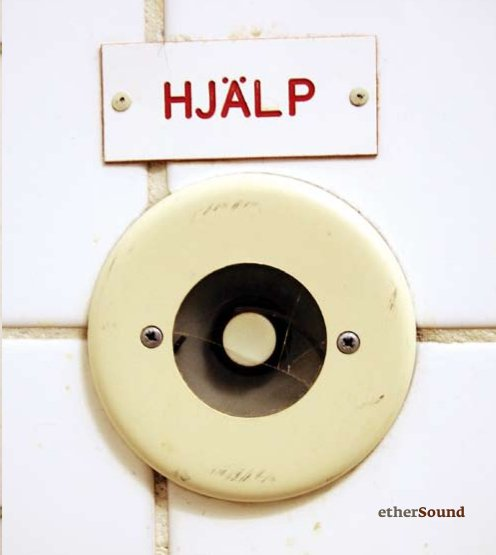
\includegraphics[width=\linewidth]{img/ethers-cover}
  \caption{Cover for Kopasetic Productions 024, \emph{etherSound}}
  \label{fig:ether-cover}
\end{wrapfigure}
All the messages sent during that hour were stored along with the
absolute time at which they were received and just as their contents were
used that day to generate computer originated sounds have they been
used in this recording to generate the electro-acoustic track. The
messages appear in the exact same order and at the exact same relative
time position as they were received in the concert and in that sense, this
recording is a mirror image in time of that evening. Those who
participated in the concert also participate on this
recording. The third track, \emph{luc:)knallal}, on this record is the
representation in time of Blomqvist's \emph{Flight}
(though time is the only relation) and is hence unaccompanied (no
electronics). About 1'20'' into the fourth track, \emph{be mean}, the
electronics re-appear and marks the beginning of the May 8, 2004 
\emph{Jeriko} performance.

While recording this CD, the electronic track became like a third
player to me and Peter. Despite its static nature, it appeared as a
quite dynamic agent that mediated the `presence' of the concert
participants, the other musicians and the ambiance. This presence
made it necessary for us to engage in discussions concerning our
musical relation to these distant performers.

In another setting we might have chosen strategies that would allow
for a more free approach but in this case we had to respect the absent
players (or there would be no point in doing the record in this way)
at the expense of our own freedom. We had to give up ourselves (our
\emph{egos}) in order to allow place for the collective. The
collective introduced the authenticity that we had to relate to.

A recording is a simulation of a musical performance and in the case
of improvised music it is simulated improvisation (though not
necessarily less authentic). In some cases I would be
inclined to say that a recording is a work type of its own, only
vaguely related to the music it simulates. This particular recording
is a two fold simulation: It is a simulation of the performance of
\emph{etherSound} but it is also the simulation of interaction between
an unnamed collective force and two musicians---just as
\emph{etherSound} already in its earliest conceptions was a
simulation: A simulation of mobile phones playing music.

%%% Local Variables: 
%%% mode: latex
%%% TeX-master: "../ethersound-cd"
%%% End: 
